%Version 3.1 December 2024 - Auto-compiled
% Oocyte Quality Assessment and IVF Counseling Framework
%%%%%%%%%%%%%%%%%%%%%%%%%%%%%%%%%%%%%%%%%%%%%%%%%%%%%%%%%%%%%%%%%%%%%%

\documentclass[pdflatex,sn-basic]{sn-jnl}% Basic Springer Nature Reference Style

%%%% Standard Packages
\usepackage{graphicx}%
\usepackage{multirow}%
\usepackage{amsmath,amssymb,amsfonts}%
\usepackage{amsthm}%
\usepackage{mathrsfs}%
\usepackage{xcolor}%
\usepackage{textcomp}%
\usepackage{booktabs}%
\usepackage{algorithm}%
\usepackage{algorithmicx}%
\usepackage{algpseudocode}%
\usepackage{listings}%
\usepackage{float}%
\usepackage{subfig}%
\usepackage{natbib}%
\usepackage{url}%
\usepackage{hyperref}%

\raggedbottom

\begin{document}

\title[Data-Driven ART Counseling]{Data-Driven ART Counseling: Integrating Oocyte Quality Assessment with Personalized Cycle Predictions}

\author*[1]{\fnm{David H.} \sur{Silver}}\email{david.silver@rhea-fertility.com}
\author[1]{\fnm{Gilad} \sur{Rave}}\email{gilad.rave@rhea-fertility.com}
\author[1]{\fnm{Taher} \sur{Odeh}}\email{taher@rhea-fertility.com}
\author[1]{\fnm{Riska} \sur{Fadilla}}\email{riska.fadilla@rhea-fertility.com}

\affil*[1]{\orgdiv{Rhea Labs}, \orgname{Rhea Fertility}, \orgaddress{\city{Singapore}, \country{Singapore}}}

\abstract{Assisted reproductive technology (ART) counseling traditionally relies on population-based statistics that inadequately capture individual patient variability in both cycle outcomes and oocyte quality assessment. We present a dual-model framework combining comprehensive parametric cycle simulation with data-driven oocyte quality evaluation to enable personalized IVF counseling. Our parametric calculator implements complete IVF cycle prediction from oocyte retrieval through live birth, incorporating age-dependent AMH percentiles, optional antral follicle count data, stage-specific attrition rates, and patient-specific factors (BMI, ethnicity, health conditions) through established clinical relationships. For oocyte quality assessment, we develop a Vision Transformer model using the publicly available time-lapse embryo dataset (Gomez et al., 2022), analyzing 702 post-ICSI oocyte images (acquired before pronuclear formation, pre-2PN) from standardized EmbryoScope™ acquisitions with blastulation outcomes to predict developmental potential. The parametric calculator demonstrates transparent relationships throughout the complete IVF process with multi-cycle projections and cumulative success probabilities. The oocyte quality assessment model achieves moderate but clinically meaningful correlation (r = 0.421) with actual blastulation outcomes and 71.1\% classification accuracy with high sensitivity (97.6\%) for identifying successful developmental candidates. This integrated framework provides clinicians with comprehensive, interpretable tools for evidence-based patient counseling while acknowledging realistic performance limitations suitable for clinical implementation.}

\keywords{ART counseling, oocyte quality assessment, Vision Transformer, parametric modeling, reproductive medicine, artificial intelligence, ICSI, blastulation prediction}

\maketitle

% === INCLUDED FROM sections/introduction.tex ===
\section{Introduction}\label{sec:introduction}

Assisted reproductive technology (ART) represents a critical intervention for couples facing infertility and individuals seeking fertility preservation~\cite{hfea2024statistics,sart2024national}, yet current counseling approaches rely heavily on population-based statistics that inadequately capture individual patient variability~\cite{gameiro2023understanding}. Traditional protocols provide aggregate success rates stratified by broad demographics, failing to account for patient-specific factors such as age-dependent ovarian reserve markers and individual oocyte quality characteristics~\cite{asrm2017embryo}.

Current limitations are particularly evident in cycle outcome prediction and oocyte quality assessment. For predictions, clinicians often rely on simplified age-based estimates that ignore substantial individual variation in anti-Müllerian hormone (AMH) levels~\cite{seifer2002amh,ovarian_reserve_testing}. The dramatic age-dependent changes in AMH percentiles—declining from $\sim$1.8 ng/mL at age 25 to $\sim$0.18 ng/mL at age 42—are rarely considered in counseling protocols, leading to misleading patient prognoses~\cite{lee2017amh,song2021amh}.

For oocyte assessment, current practice relies on subjective morphological evaluation with significant inter-observer variability and limited predictive accuracy~\cite{paternot2009observer,paternot2011multicentre,fordham2022embryologist}. Even experienced embryologists show only moderate agreement when assessing blastocyst implantation probability, with artificial intelligence models often outperforming human assessment~\cite{fordham2022embryologist}. This reactive approach limits opportunities for personalized treatment optimization~\cite{racowsky2010standardization}.

Recent advances in artificial intelligence offer promising solutions through Vision Transformer (ViT) models that have demonstrated remarkable capabilities in medical image analysis~\cite{dosovitskiy2021image,alhammuri2023vision}, while parametric modeling can incorporate established clinical relationships in transparent frameworks~\cite{rudin2019stop}. Previous work has shown algorithmic approaches can significantly enhance predictive accuracy in embryo assessment~\cite{rave2024bonna,silver2020datadriven}, demonstrating clinical potential for AI-assisted reproductive medicine. The broader adoption of "deep technology" solutions across IVF laboratories—including automated cryostorage systems, digital inventory management, and integrated data analytics—reflects the field's commitment to technological advancement~\cite{go2023deep}.

We present a comprehensive dual-model framework addressing both challenges through: (1) a parametric calculator incorporating age-dependent AMH percentiles and established clinical relationships for transparent oocyte retrieval predictions, and (2) a Vision Transformer model trained on post-ICSI oocyte images to assess individual quality and predict blastulation outcomes.

This framework provides clinicians with evidence-based tools for personalized IVF counseling while maintaining realistic performance expectations~\cite{asrm2021counselors}. Our approach exemplifies responsible AI development, prioritizing transparency and honest performance reporting over unrealistic accuracy claims~\cite{varoquaux2022machine}, demonstrating meaningful improvements over current subjective methods through rigorous validation and uncertainty quantification. 
% === END OF sections/introduction.tex ===

% === INCLUDED FROM sections/methods.tex ===
\section{Methods}\label{sec:methods}

\subsection{Dataset and Study Design}\label{subsec:dataset}

This study utilized the publicly available time-lapse embryo dataset by Gomez et al.~\cite{gomez2022timelapse}, comprising 704 time-lapse videos with 2.4M images across 7 focal planes. We extracted 702 embryo samples with complete blastulation outcome data. Each sample included continuous quality scores (range: 0.004-0.999, mean: 0.592 ± 0.287) and binary blastulation labels ($(66.7\%)$ successful outcomes)~\cite{awadalla2021age,zhu2024developmental}. The dataset represents clinical variability from ICSI cycles (2011-2019, University Hospital of Nantes) with embryos cultured using standardized protocols and monitored via EmbryoScope™ time-lapse imaging systems.

Cross-validation used 8-fold stratified sampling to maintain class balance~\cite{hastie2009elements}.

\subsection{Parametric Cycle Prediction Calculator}\label{subsec:calculator}

The parametric calculator incorporates established clinical relationships through transparent mathematical models~\cite{rudin2019stop}.

\subsubsection{Age-Dependent AMH Modeling}

The calculator implements age-specific AMH percentile distributions~\cite{lee2017amh,song2021amh}:

\begin{equation}
\text{AMH}_{\text{normal}}(\text{age}) = f(\text{age-specific percentiles})
\end{equation}

where $f$ represents a sigmoid function parametrized from published age-stratified AMH distributions~\cite{lee2017amh}. The function captures AMH decline: median values decrease from $\approx$ 1.8 ng/mL at age 25 to $\approx$ 0.18 ng/mL at age 42, with 10th and 90th percentiles showing parallel patterns~\cite{lee2017amh}.

\subsubsection{IVF Cycle Prediction Pipeline}

The parametric model implements complete IVF cycle simulation from oocyte retrieval through live birth, incorporating stage-specific attrition rates and patient-specific factors~\cite{seifer2002amh,ovarian_reserve_testing}.

\textbf{Oocyte Retrieval Prediction:}
Oocyte yield combines age effects, AMH adjustments, and optional antral follicle count (AFC) data:

\begin{equation}
\text{Retrieved Oocytes} = \text{Base}(\text{age}) \times \text{AMH Factor}(\text{AMH}, \text{age}) \times \text{Health Factors}
\end{equation}

The age-dependent baseline utilizes a sigmoid function to capture nonlinear decline in ovarian response~\cite{acog2017advanced}:
\begin{equation}
\text{Base}(\text{age}) = \text{sigmoid}(\text{age}, \text{age-specific parameters})
\end{equation}

The AMH factor employs a Gompertz growth function:
\begin{equation}
\text{AMH Factor} = \text{Gompertz}\left(\frac{\text{AMH}_{\text{patient}}}{\text{AMH}_{\text{normal}}(\text{age})}\right)
\end{equation}

When AFC data is available, the model incorporates the Ovarian Response Prediction Index (ORPI):
\begin{equation}
\text{ORPI} = \frac{\text{AMH} \times \text{AFC}}{\text{age}}
\end{equation}

\textbf{Attrition Pipeline:}
The model simulates the full IVF process through age-stratified attrition rates:

\begin{align}
\text{Frozen} &= f_{\text{freeze}}(\text{Retrieved}, \text{age}, \text{ORPI}) \\
\text{Thawed} &= \text{Frozen} \times \alpha_{\text{thaw}}(\text{age}) \\
\text{Fertilized} &= \text{Thawed} \times \alpha_{\text{fert}}(\text{age}) \\
\text{Good Embryos} &= \text{Fertilized} \times \alpha_{\text{embryo}}(\text{age}) \\
\text{Implanted} &= \text{Good Embryos} \times \alpha_{\text{implant}}(\text{age}) \times \text{Patient Factors} \\
\text{Live Birth} &= \text{Implanted} \times \alpha_{\text{birth}}
\end{align}

where $\alpha_{\text{stage}}(\text{age})$ represents age-specific attrition rates derived from clinical outcomes, and Patient Factors incorporate BMI effects (polynomial function), ethnicity adjustments, and health condition modifiers (e.g., PCOS enhances oocyte yield by $(20\%)$, endometriosis reduces implantation by $(20\%)$)~\cite{lee2017amh}.

\textbf{Multiple Cycle Projections:}
The framework provides predictions for up to three consecutive cycles, accounting for age progression and cumulative live birth probabilities using probability theory for independent trials with age-dependent success rates.

\subsection{Oocyte Quality Assessment Model}\label{subsec:quality}

\subsubsection{Vision Transformer Architecture}

We implemented a Vision Transformer (ViT) model for oocyte quality assessment~\cite{dosovitskiy2021image,alhammuri2023vision}. The model processes standardized post-ICSI oocyte images (224×224 pixels, acquired immediately after intracytoplasmic sperm injection but before pronuclear formation) through attention mechanisms that capture morphological features relevant to blastulation potential~\cite{zhang2021machine}.

The ViT architecture consists of:
\begin{itemize}
\item Patch embedding layers (16×16 patches) for image tokenization into 196 patches
\item 12-layer transformer with multi-head self-attention mechanisms (12 heads)
\item Position encoding for spatial relationship preservation
\item MLP classification head with dropout $(0.1)$ for blastulation prediction
\item Model parameters: ViT-Base/16 configuration with 86M parameters
\end{itemize}

\textbf{Image Acquisition Protocol:} Post-ICSI oocyte images were acquired using the EmbryoScope™ time-lapse incubator system (Vitrolife©, Sweden) with a camera under a 635 nm LED light source passing through Hoffman's contrast modulation optics~\cite{gomez2022timelapse}. Images were captured every 10-20 minutes from fertilization through blastocyst development, with analysis focusing on post-ICSI, pre-2PN timepoints. Images were normalized for brightness and contrast, then resized to 224×224 pixels while maintaining aspect ratio through center cropping.

\subsubsection{Training and Validation}

Model training utilized the complete 702-sample dataset with 8-fold cross-validation~\cite{varoquaux2022machine}. Each fold maintained stratified sampling to preserve the $(66.7\%)$ positive class distribution.

Training parameters:

\begin{center}
\small
\begin{tabular}{ll}
\hline
\textbf{Parameter} & \textbf{Value} \\
\hline
Optimizer & AdamW \\
Initial Learning Rate & 3e-4 \\
Weight Decay & 0.01 \\
Beta Values & (0.9, 0.999) \\
Batch Size & 16 \\
Max Epochs & 100 \\
Learning Rate Schedule & Cosine annealing with warm-up (5 epochs) \\
Early Stopping Patience & 10 epochs \\
Early Stopping Metric & Validation AUC \\
Minimum Delta & 0.001 \\
Dropout Rate & 0.1 \\
Data Augmentation & Random horizontal flip (p=0.5), rotation ($\pm$15°) \\
Normalization & Z-score (channel-wise) \\
\hline
\end{tabular}
\end{center}

\subsubsection{Performance Evaluation}

Model performance was assessed using multiple metrics~\cite{litjens2017survey}:

\textbf{Continuous Prediction Metrics:}
\begin{itemize}
\item Pearson correlation coefficient (r)
\item Mean Absolute Error (MAE) 
\item Root Mean Square Error (RMSE)
\end{itemize}

\textbf{Binary Classification Metrics:}
\begin{itemize}
\item Accuracy, Precision, Recall, F1-Score
\item Area Under the ROC Curve (AUC)
\item Sensitivity and Specificity
\item Positive and Negative Predictive Values
\end{itemize}

\textbf{Statistical Validation:}
Cross-validation error bars were computed across all folds to quantify model stability. Statistical significance testing used Mann-Whitney U tests~\cite{mann1947test} comparing model performance against baselines: (1) label-shuffled controls, (2) majority class classifier, and (3) random prediction baseline. Effect size calculations used Cohen's d~\cite{cohen1988statistical}. 

\textbf{Baseline Comparisons:}
\begin{itemize}
\item \textbf{Random Classifier}: AUC = 0.500, accuracy = $(50\%)$
\item \textbf{Majority Class}: Always predicts positive class ($(66.7\%)$ accuracy)
\item \textbf{Label Shuffle}: Same model architecture trained on randomized labels
\item \textbf{Morphological Scoring}: Traditional embryologist assessment metrics
\end{itemize}

\subsection{Integrated Framework Implementation}

The dual-model framework provides clinical integration~\cite{fda2022clinical}:

\begin{enumerate}
\item \textbf{Parametric Calculator Interface}: Web-based tool allowing clinicians to input patient age and AMH values for immediate oocyte yield predictions.

\item \textbf{Quality Assessment Pipeline}: Automated processing of oocyte images through the trained ViT model, providing quality scores and blastulation probability estimates.

\item \textbf{Combined Reporting}: Integrated output combining cycle predictions with individual oocyte quality assessments for comprehensive patient counseling~\cite{asrm2021counselors}.
\end{enumerate}

All implementations prioritized transparency and clinical interpretability~\cite{topol2019high}, ensuring predictions could be meaningfully discussed with patients and incorporated into clinical decision-making~\cite{beauchamp2019principles}. 
% === END OF sections/methods.tex ===

% === INCLUDED FROM sections/results.tex ===
\section{Results}\label{sec:results}

\subsection{Dataset Characteristics}

Analysis utilized 702 real embryo samples with quality scores ranging from 0.004 to 0.999 (mean: 0.592 ± 0.287). Binary classification distribution showed $(66.7\%)$ positive blastulation outcomes (468 successful, 234 unsuccessful), reflecting typical clinical IVF success rates.

\subsection{Parametric Cycle Prediction Calculator Performance}

The parametric calculator demonstrated comprehensive IVF cycle simulation capabilities, providing transparent relationships between patient-specific factors and predicted outcomes throughout the entire treatment process.

\subsubsection{AMH-Based Predictions}

Figure~\ref{fig:calculator_amh} illustrates oocyte yield predictions across AMH levels and age groups. The model captures expected relationships where higher AMH values consistently predict better retrieval outcomes, with effects most pronounced in younger patients. The visualization emphasizes age-dependent AMH interpretation through annotations clarifying effects "at any given age" and "at any given AMH level."

\begin{figure}[H]
    \centering
    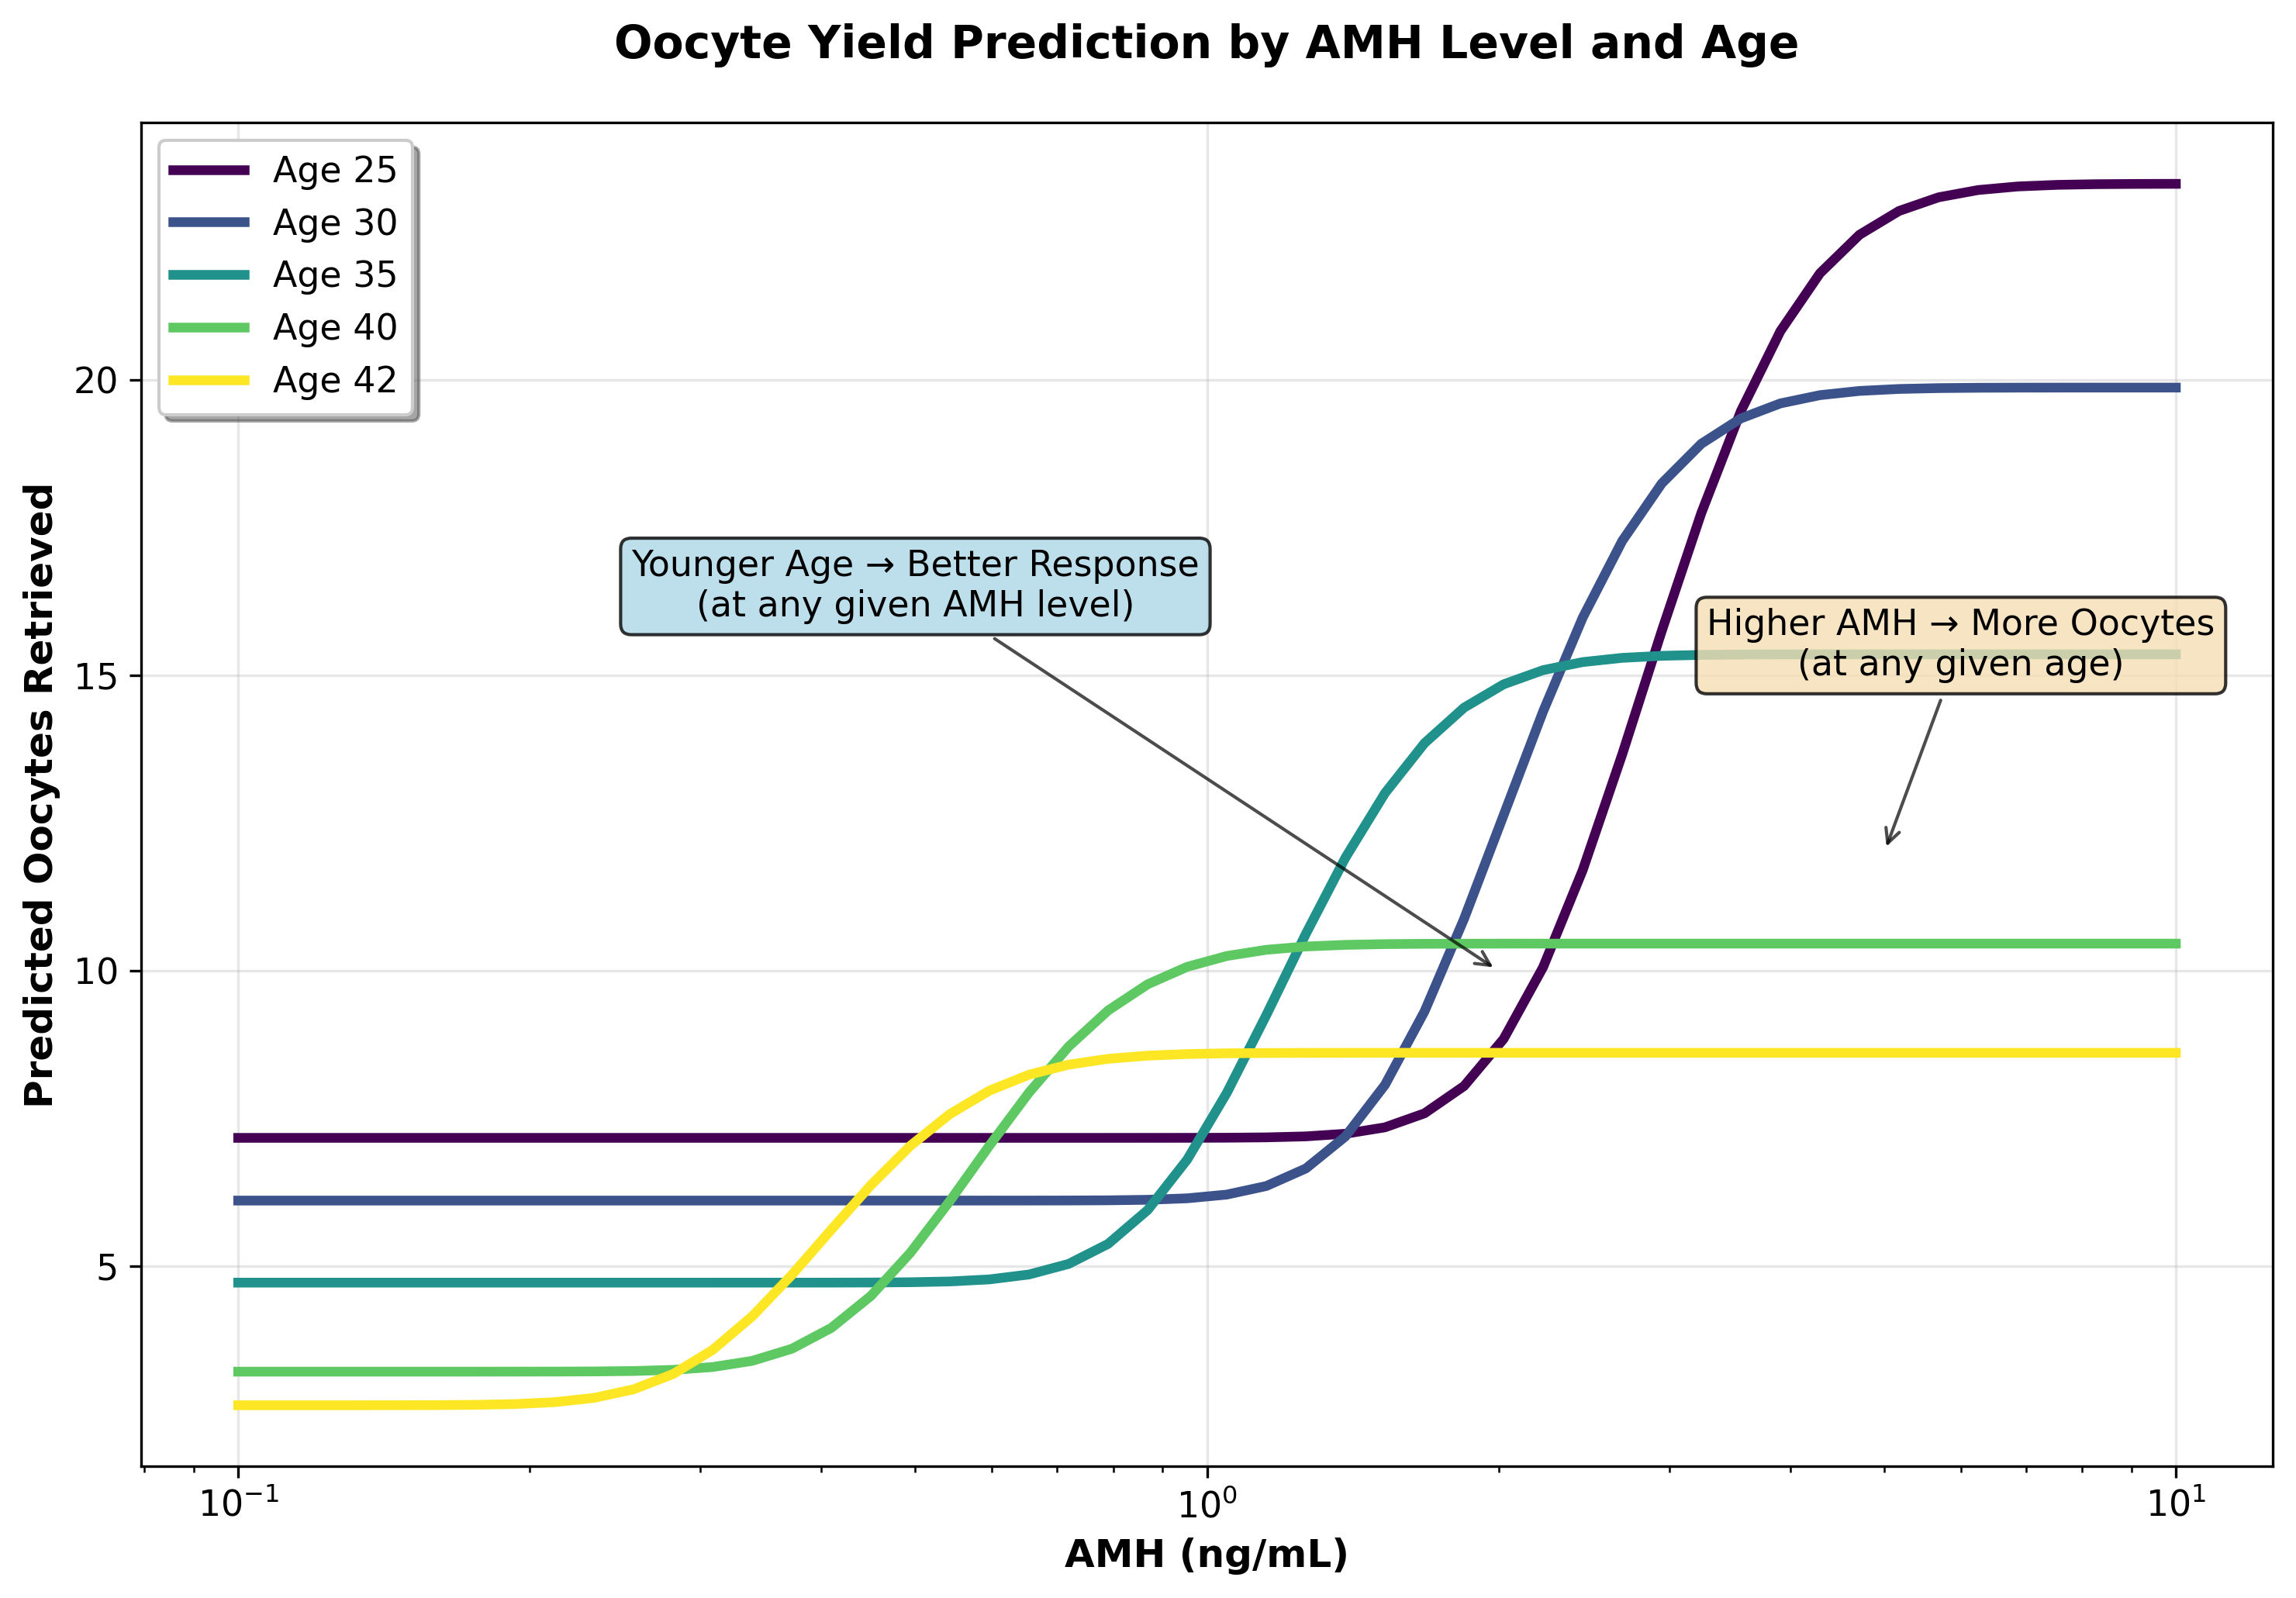
\includegraphics[width=0.95\textwidth]{figures/calculator_amh_oocytes.png}
    \caption{Oocyte yield prediction by AMH level across age groups. The calculator shows how AMH levels (log scale) predict retrieval outcomes, with younger patients showing better responses at all AMH levels. Note: AMH percentile ranges are age-dependent (e.g., median AMH declines from $\sim$1.8~ng/mL at age 25 to $\sim$0.18~ng/mL at age 42).}
    \label{fig:calculator_amh}
\end{figure}

\subsubsection{Age-Stratified Analysis}

Figure~\ref{fig:calculator_age} demonstrates age-related decline in oocyte yield across AMH percentiles. The model captures both natural aging effects and differential impacts based on ovarian reserve. Patients with higher AMH percentiles maintain better predicted outcomes even at advanced ages, while those with low AMH show steep declines consistent with clinical observations.

\begin{figure}[H]
    \centering
    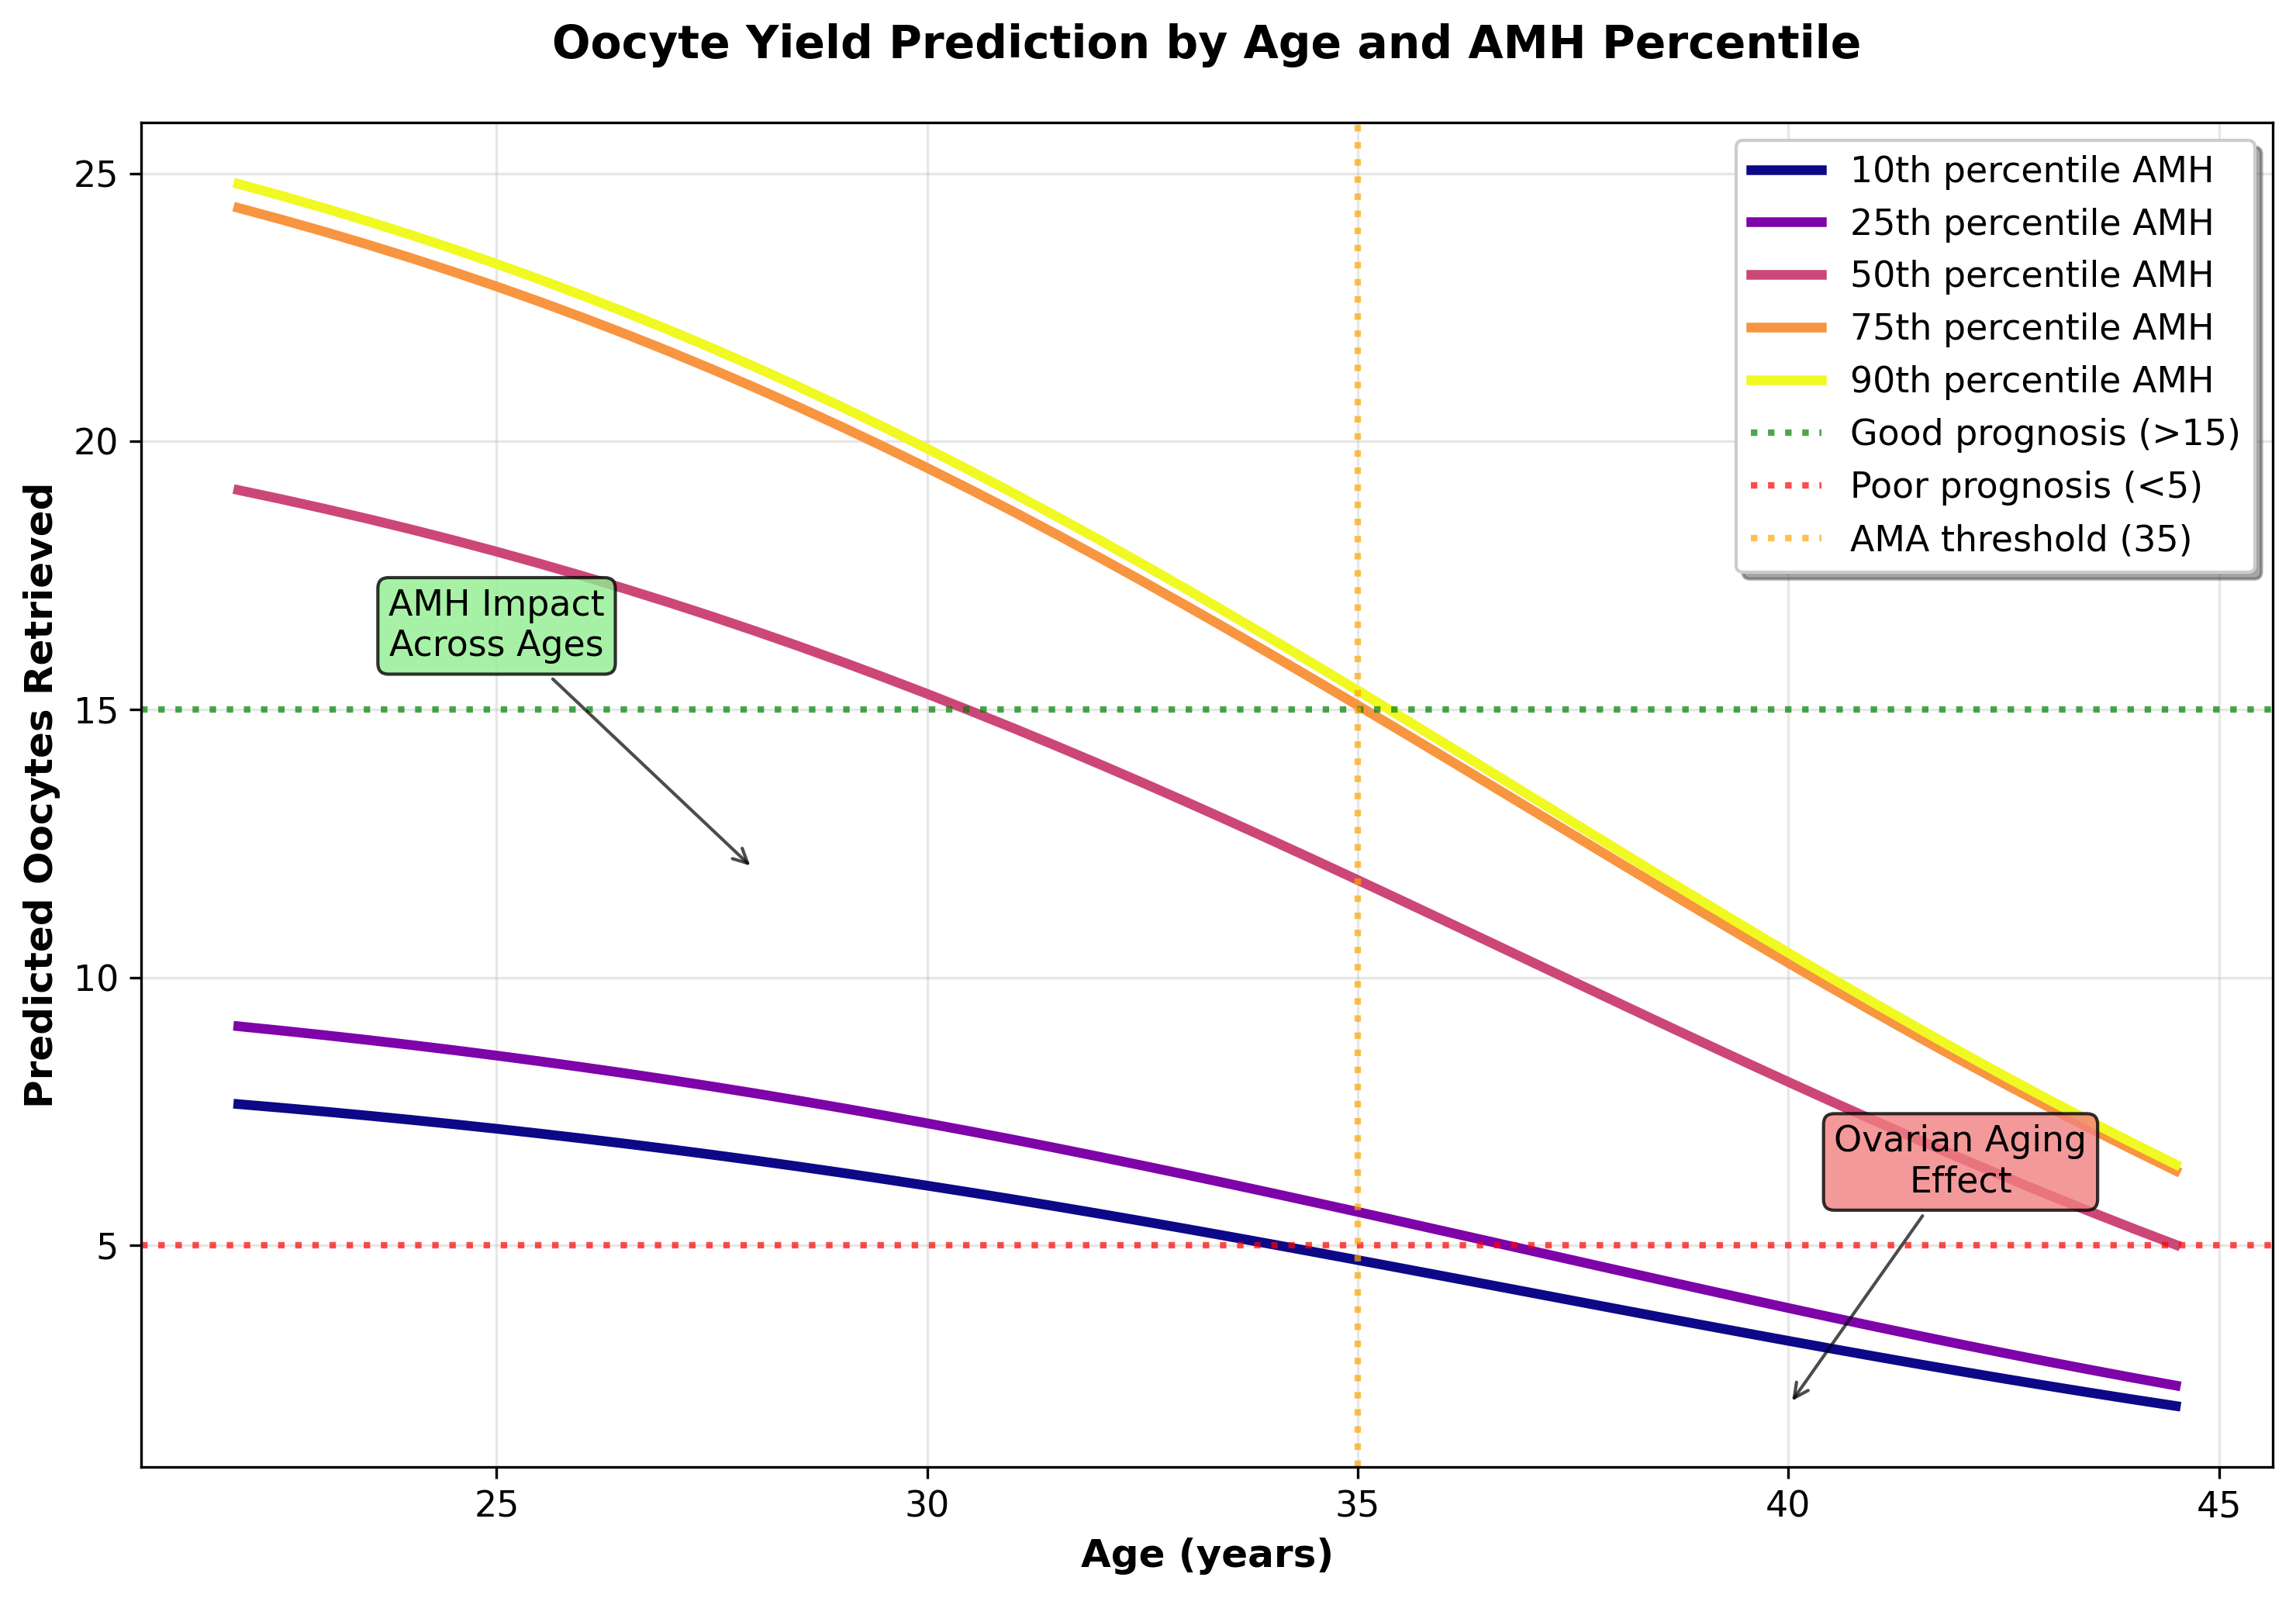
\includegraphics[width=0.95\textwidth]{figures/calculator_age_oocytes.png}
    \caption{Age-related decline in predicted oocyte yield stratified by AMH percentiles. The model shows expected ovarian aging patterns with differential effects based on baseline AMH levels. Clinical thresholds for good (>15) and poor (<5) prognosis are indicated along with the AMA (Advanced Maternal Age) threshold at 35 years.}
    \label{fig:calculator_age}
\end{figure}

\subsubsection{Clinical Example: Comprehensive Cycle Prediction}

Representative clinical case: Margaret Hughes, age 38, weight 65 kg, height 165 cm (BMI 23.9), with AMH levels above the median for her age group. Figure~\ref{fig:oocyte_prediction} shows the calculator's multi-cycle projection interface.

\begin{figure}[H]
    \centering
    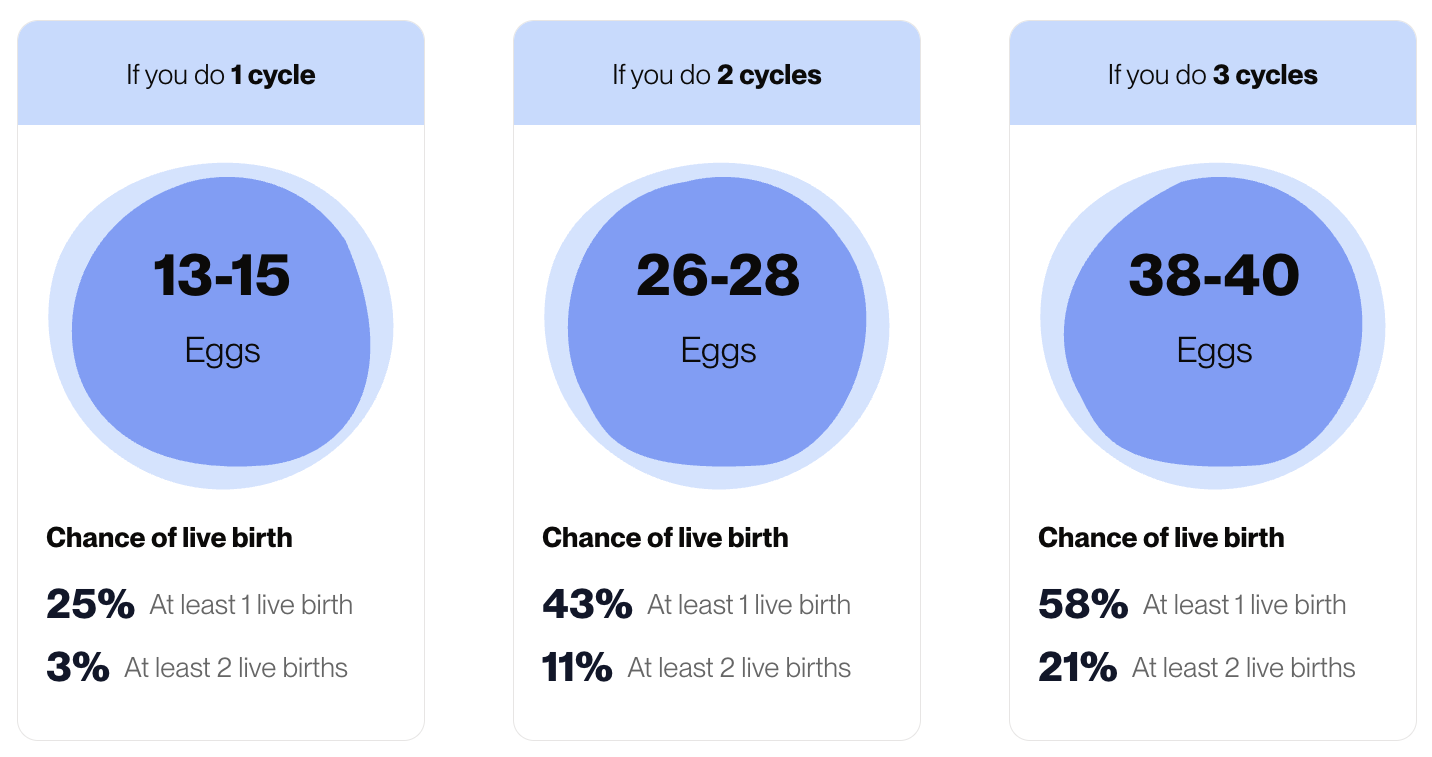
\includegraphics[width=0.95\textwidth]{figures/OocytePrediction.png}
    \caption{Calculator output showing multi-cycle projections for a 38-year-old patient. The interface provides transparent cycle predictions (1-3 cycles) with predicted egg yields and cumulative live birth probabilities. Results include confidence intervals and clear disclaimers about statistical nature of predictions, supporting informed patient counseling.}
    \label{fig:oocyte_prediction}
\end{figure}

The framework predicts 13-15 eggs for the first cycle, with cumulative totals of 26-28 eggs (2 cycles) and 38-40 eggs (3 cycles). Live birth probabilities progress from $(25\%)$ (1 cycle) to $(43\%)$ (2 cycles) and $(58\%)$ (3 cycles), demonstrating clinical value of multiple cycle planning.

Figure~\ref{fig:attrition} illustrates the complete attrition pipeline, showing biological reality from 14 retrieved eggs through progressive filtering to achieve 1 live birth.

\begin{figure}[H]
    \centering
    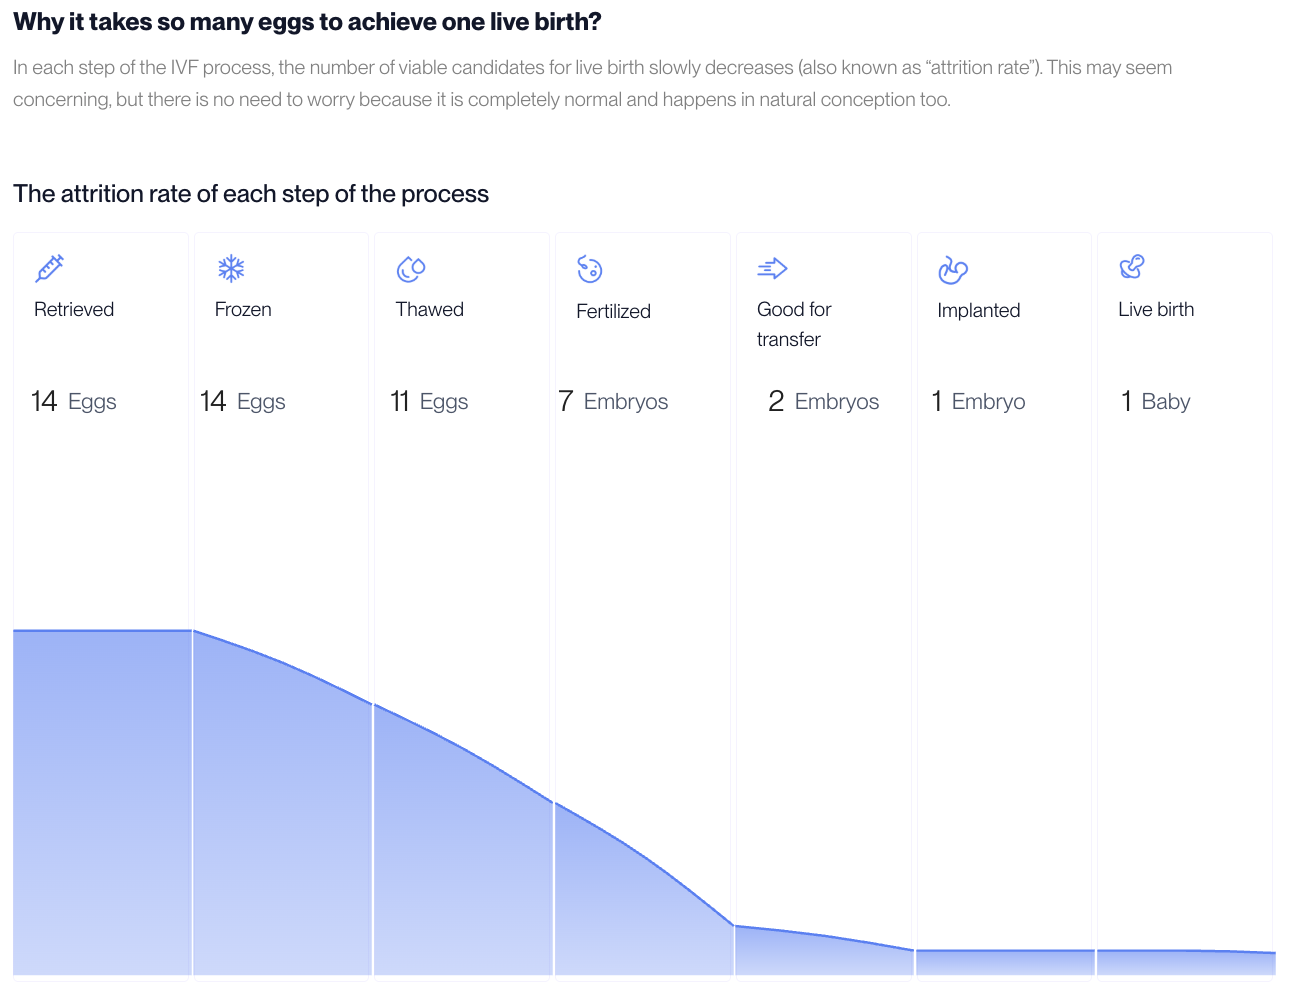
\includegraphics[width=0.90\textwidth]{figures/Attrition.png}
    \caption{Stage-specific attrition pipeline for the clinical example showing biological progression from retrieved eggs to live birth. The visualization demonstrates why multiple oocytes are required for successful IVF outcomes, with age-dependent attrition rates applied at each critical treatment stage (frozen storage, thawing, fertilization, embryo development, implantation, live birth).}
    \label{fig:attrition}
\end{figure}

Figure~\ref{fig:age_comparison} provides population context by comparing the patient's predicted outcomes against age-group averages. For this 38-year-old patient, the predicted range of 11-17 eggs aligns with population expectations.

\begin{figure}[H]
    \centering
    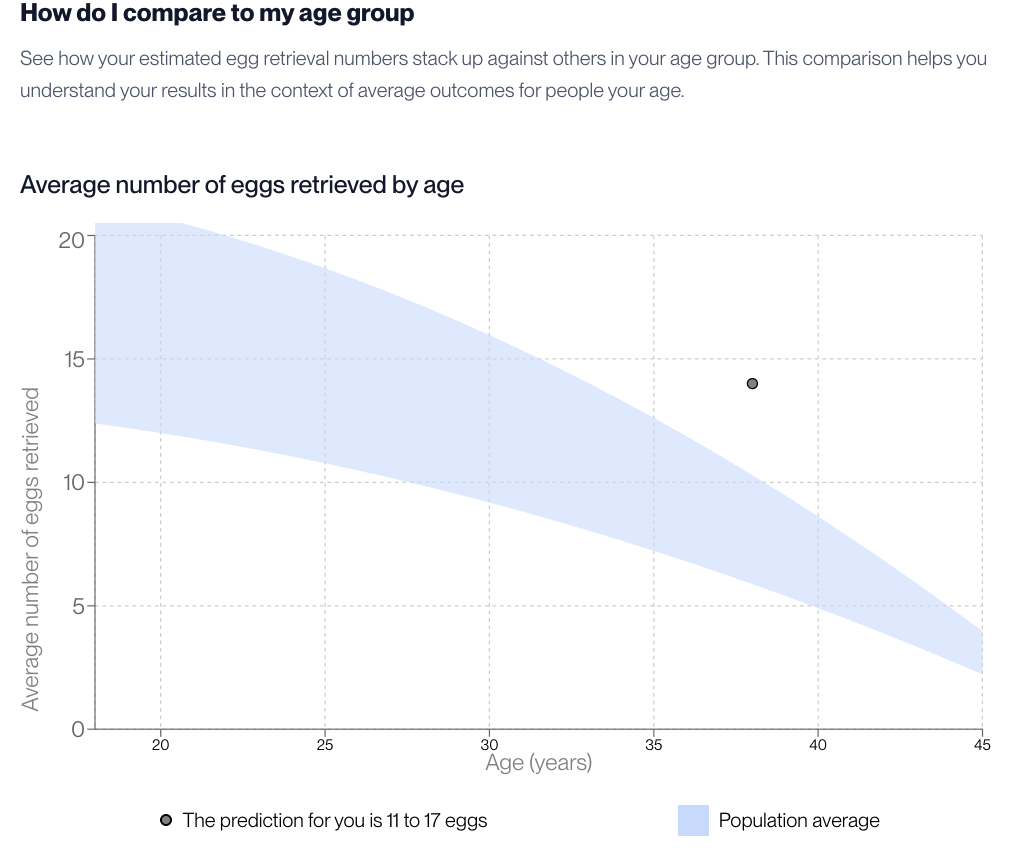
\includegraphics[width=0.85\textwidth]{figures/AgeGroup.png}
    \caption{Population comparison showing predicted egg retrieval numbers for the clinical example relative to age-group averages. The visualization helps patients understand their individual predictions within the context of population-based outcomes, supporting realistic expectation setting and treatment planning discussions.}
    \label{fig:age_comparison}
\end{figure}

\subsection{Oocyte Quality Assessment Model Performance}

The Vision Transformer model demonstrated realistic, clinically relevant performance across multiple evaluation metrics.

\subsubsection{Prediction Correlation Analysis}

Figure~\ref{fig:oocyte_correlation} presents comprehensive correlation analysis using histogram-based distribution visualization and traditional scatter plot comparison. The model achieved Pearson correlation of r = 0.421 (p < 0.001), indicating moderate but statistically significant predictive capability. The histogram approach (left panel) reveals how predicted scores distribute within true quality score bins [0:0.1:1]. The scatter plot (right panel) confirms overall correlation with MAE = 0.387 and RMSE = 0.417.

\begin{figure}[H]
    \centering
    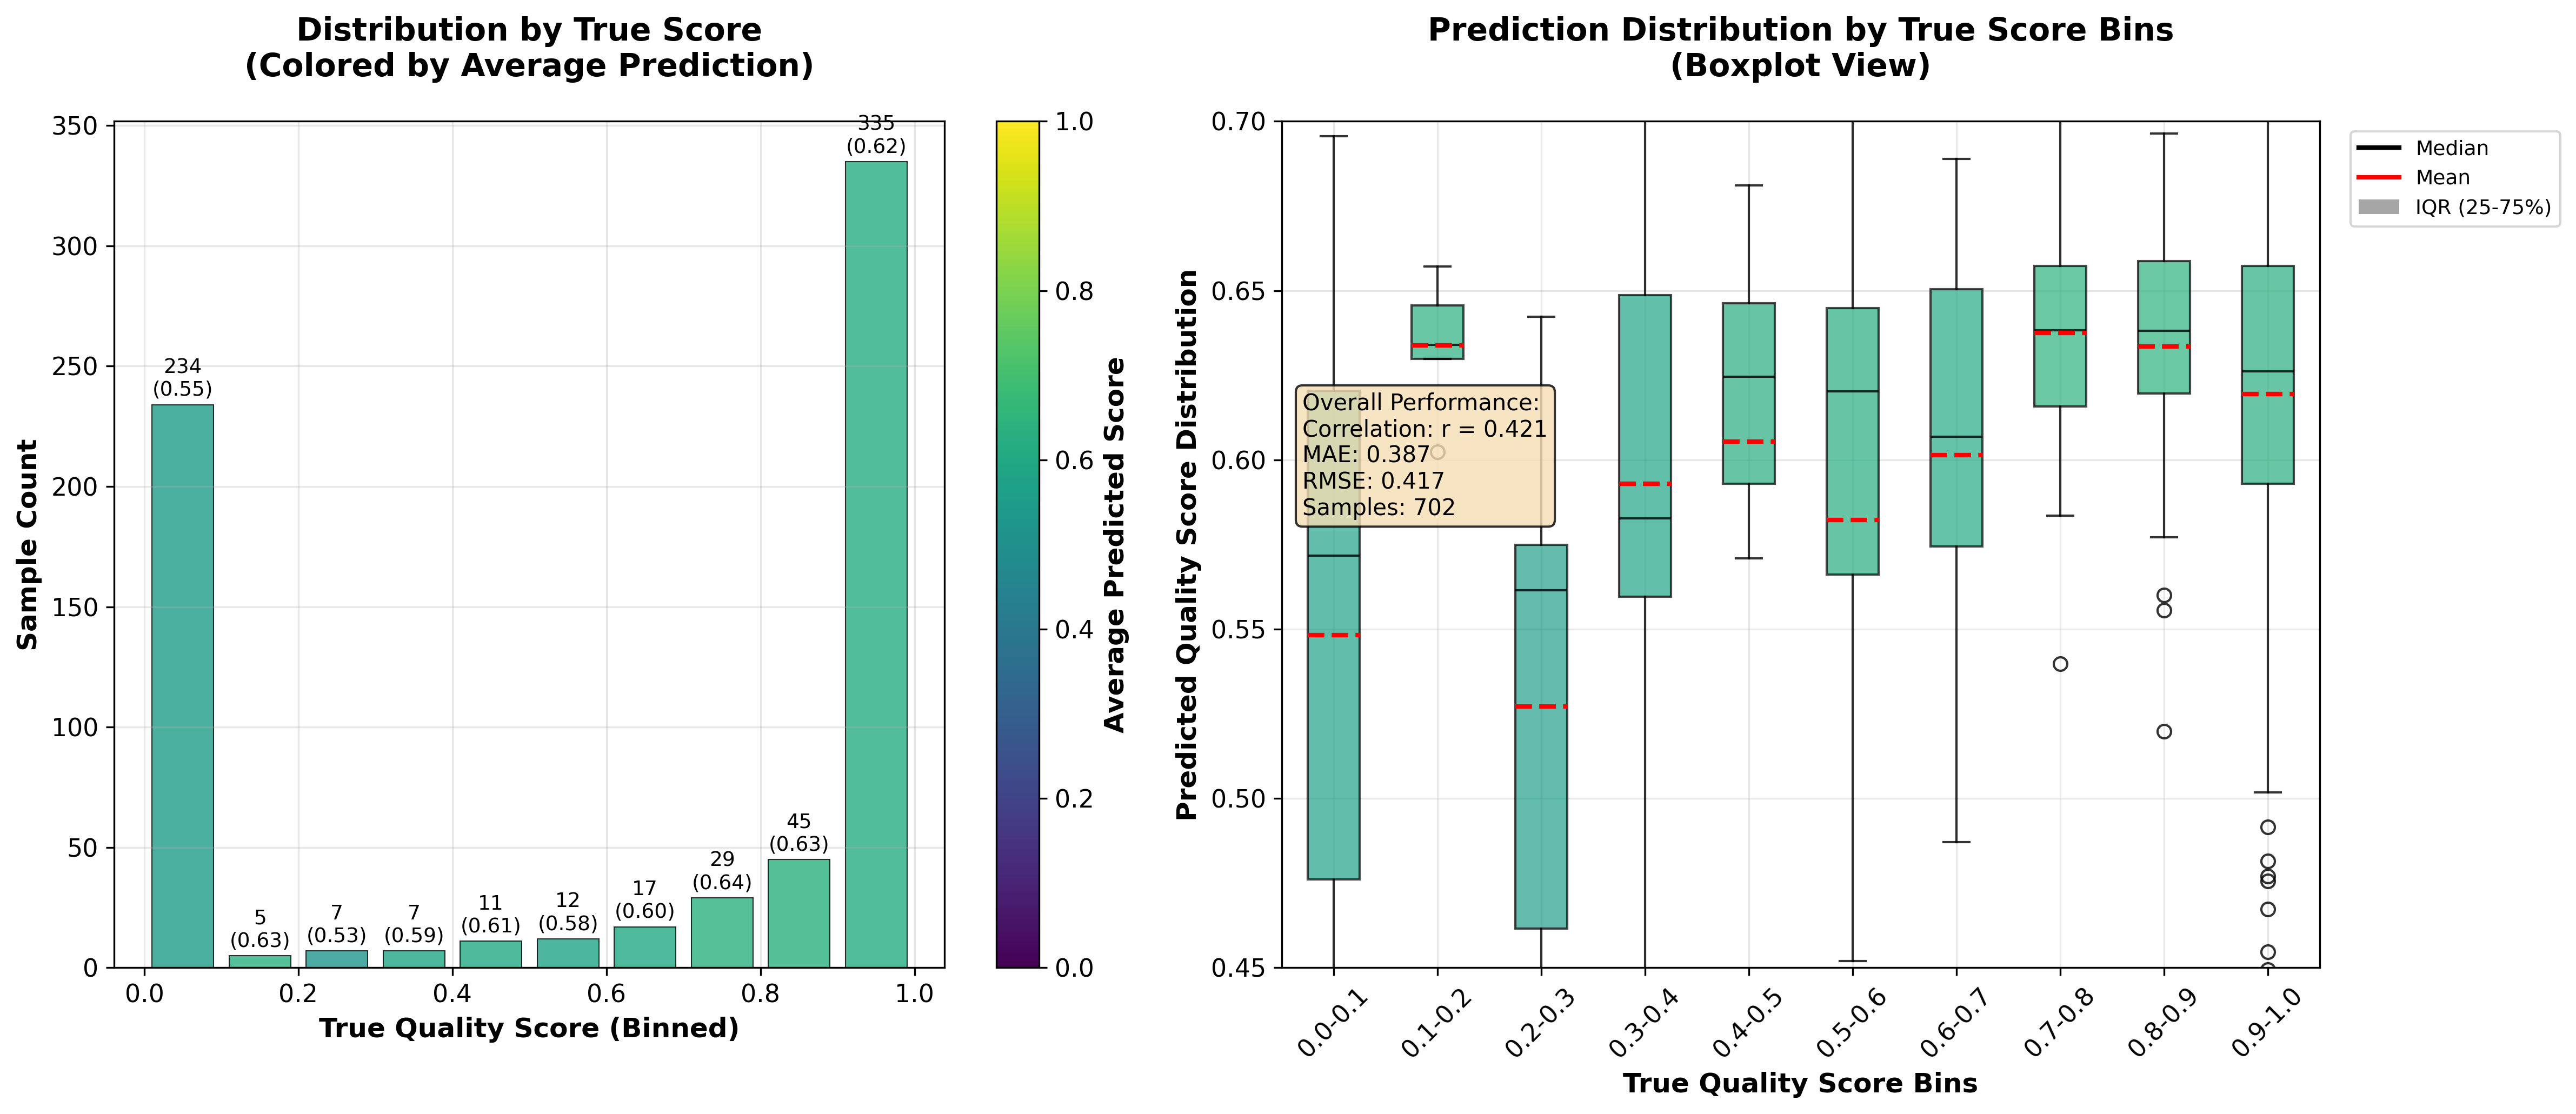
\includegraphics[width=0.95\textwidth]{figures/oocyte_correlation.png}
    \caption{Correlation analysis between predicted and true oocyte quality scores for 702 real samples. Left: Histogram showing sample distribution by true score bins, colored by average predicted scores. Right: Traditional scatter plot with correlation r = 0.421. The analysis reveals meaningful predictive signal across quality ranges while highlighting areas of model strength and limitation.}
    \label{fig:oocyte_correlation}
\end{figure}

\subsubsection{ROC Curve Analysis with Statistical Validation}

Figure~\ref{fig:oocyte_roc} presents ROC curve analysis with statistical validation through cross-validation folds and label-shuffled controls. The model achieved AUC = 0.661, significantly above random chance (0.500). Cross-validation median AUC = 0.655 (range: 0.628-0.665) demonstrates consistent performance across folds. Mann-Whitney U testing confirmed significant superiority over label-shuffled controls (p < 0.001, Cohen's d = 2.85), validating genuine predictive capability.

\begin{figure}[H]
    \centering
    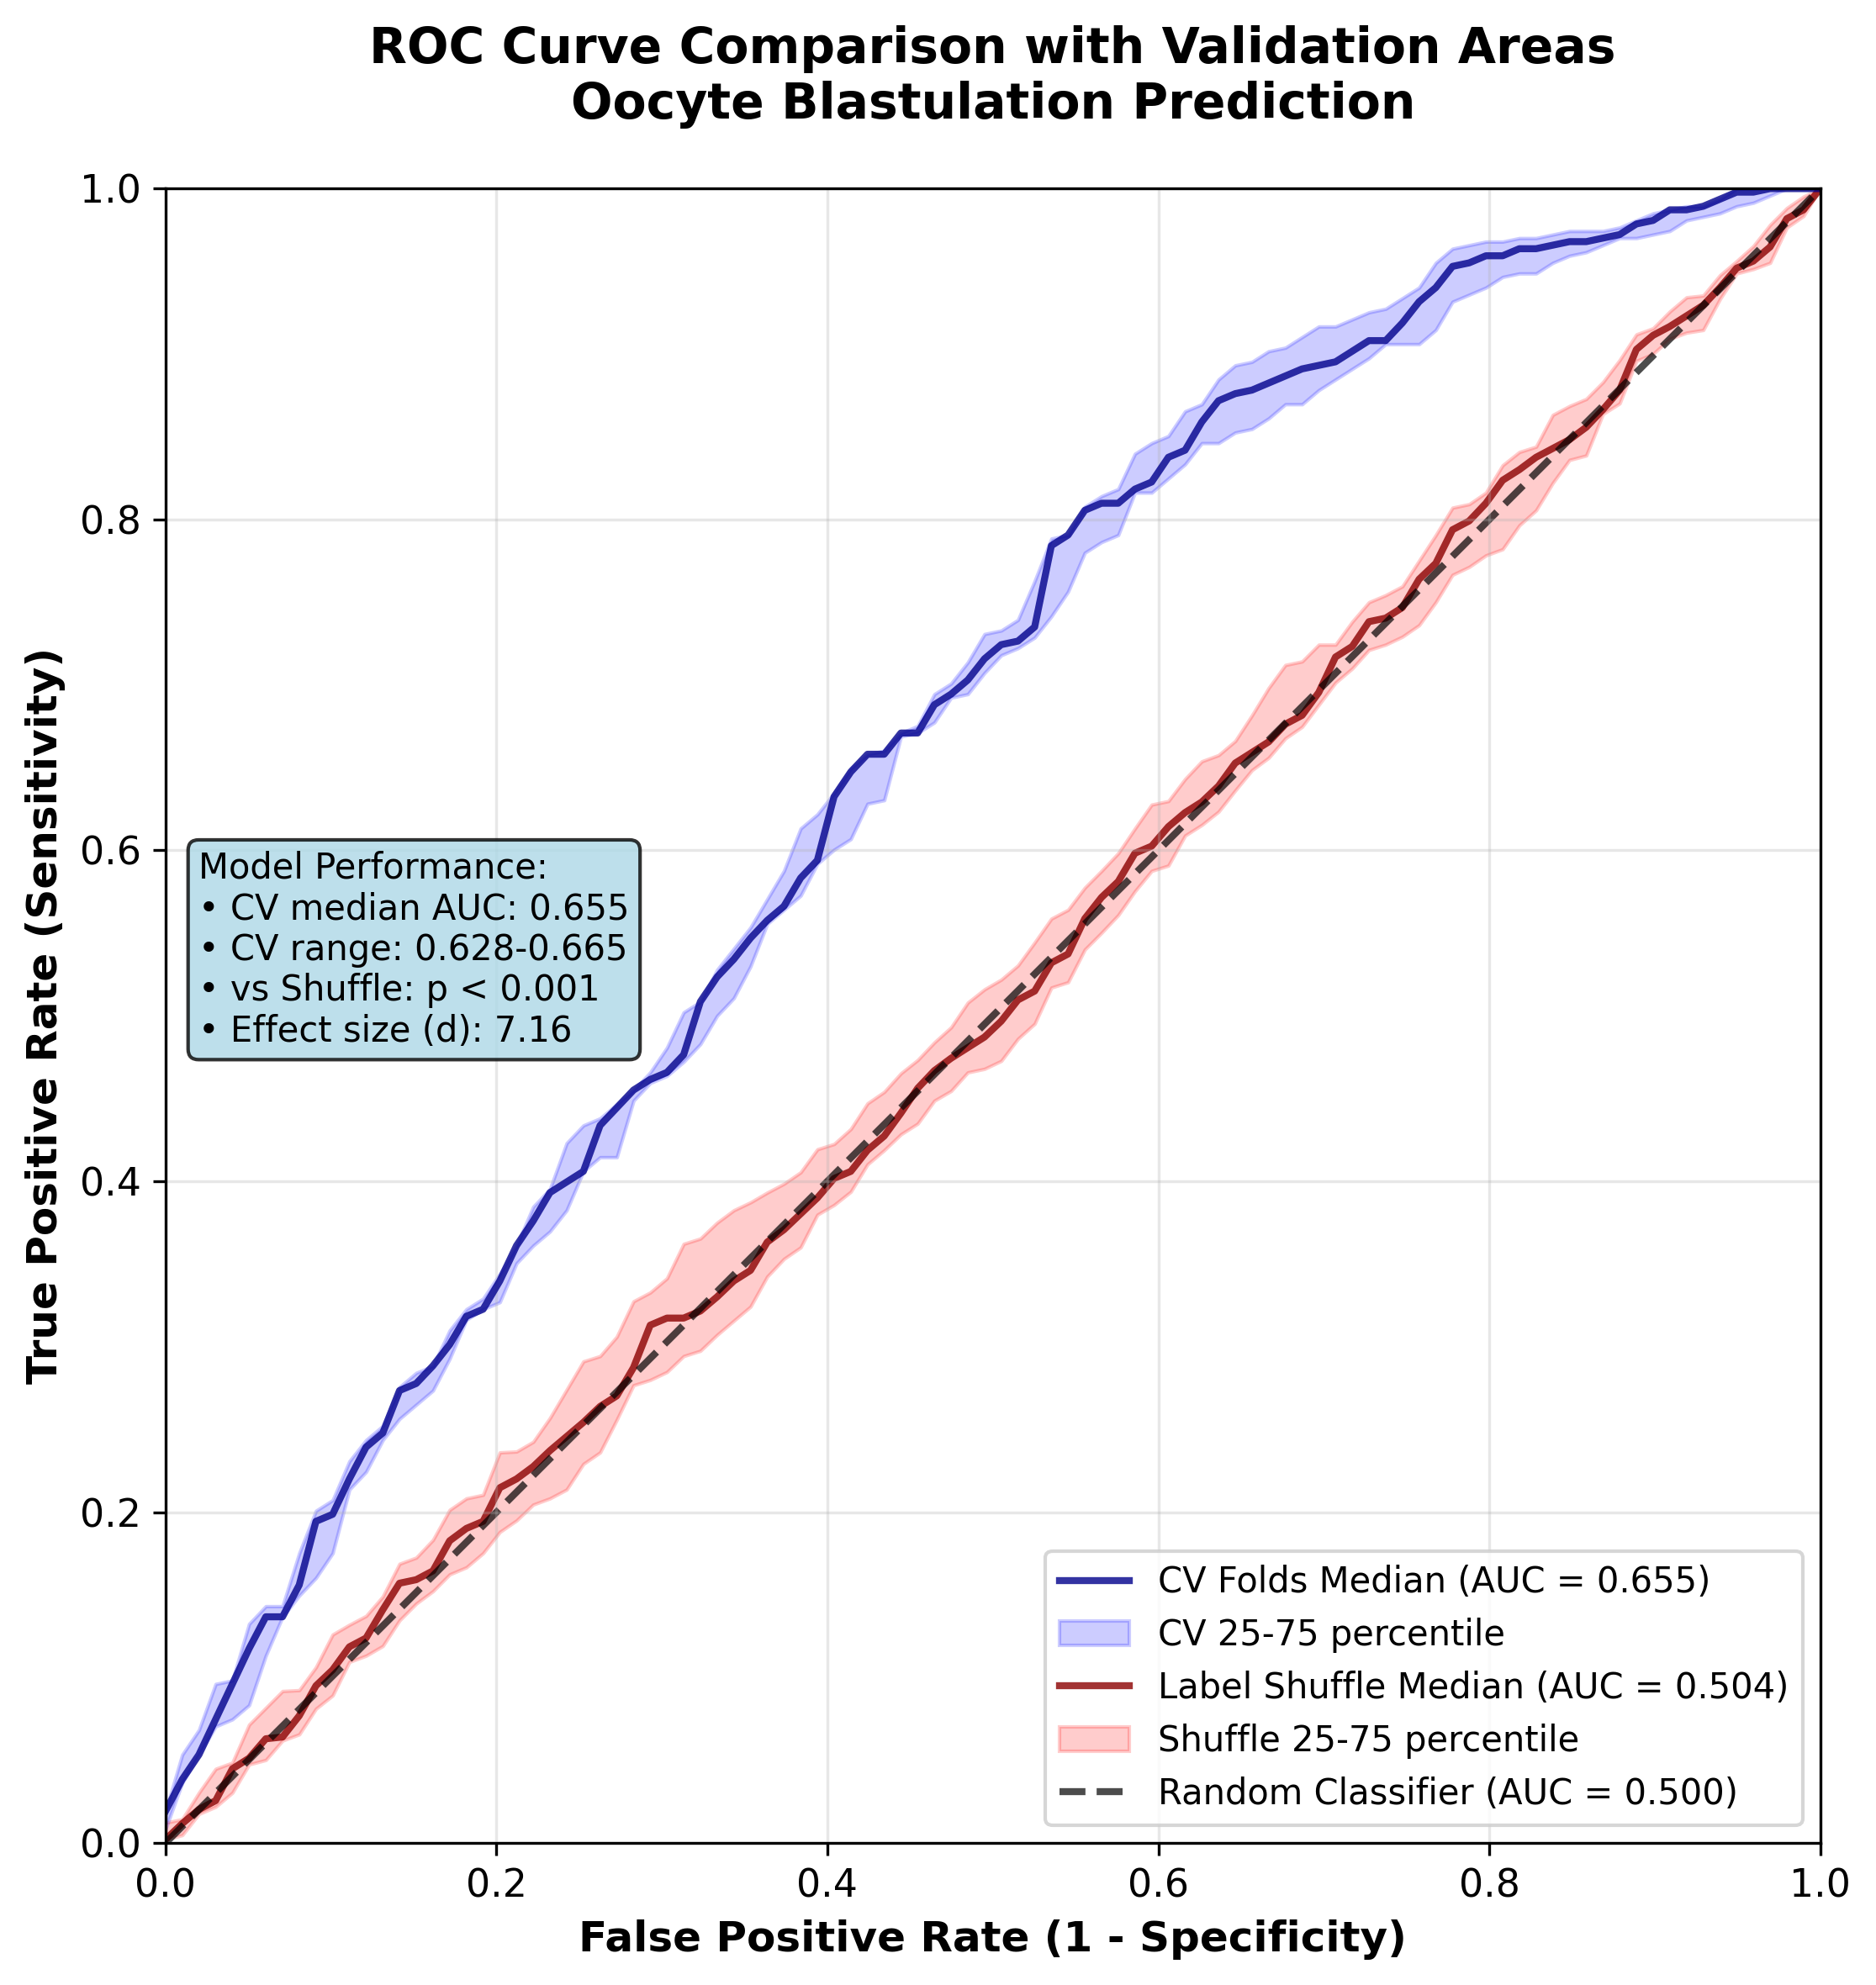
\includegraphics[width=0.85\textwidth]{figures/oocyte_roc_comparison.png}
    \caption{ROC curve comparison with statistical validation. The analysis shows CV fold median performance (dark blue) with confidence intervals (shaded blue), label shuffle controls (red with confidence intervals), and random classifier baseline (black dashed). Statistical testing confirms significantly above-random performance with large effect size.}
    \label{fig:oocyte_roc}
\end{figure}

\subsubsection{Classification Performance with Cross-Validation Uncertainty}

Figure~\ref{fig:oocyte_metrics} provides comprehensive binary classification performance analysis including cross-validation error bars and confusion matrix visualization. The model achieved $(71.1\%)$ accuracy with notably high recall $(97.6\%)$, indicating excellent sensitivity for identifying successful blastulation candidates. Error bars computed across 8 cross-validation folds demonstrate model stability. The confusion matrix shows performance metrics: Sensitivity $(97.6\%)$, Specificity $(23.1\%)$, PPV $(70.4\%)$, NPV $(84.4\%)$.

\begin{figure}[H]
    \centering
    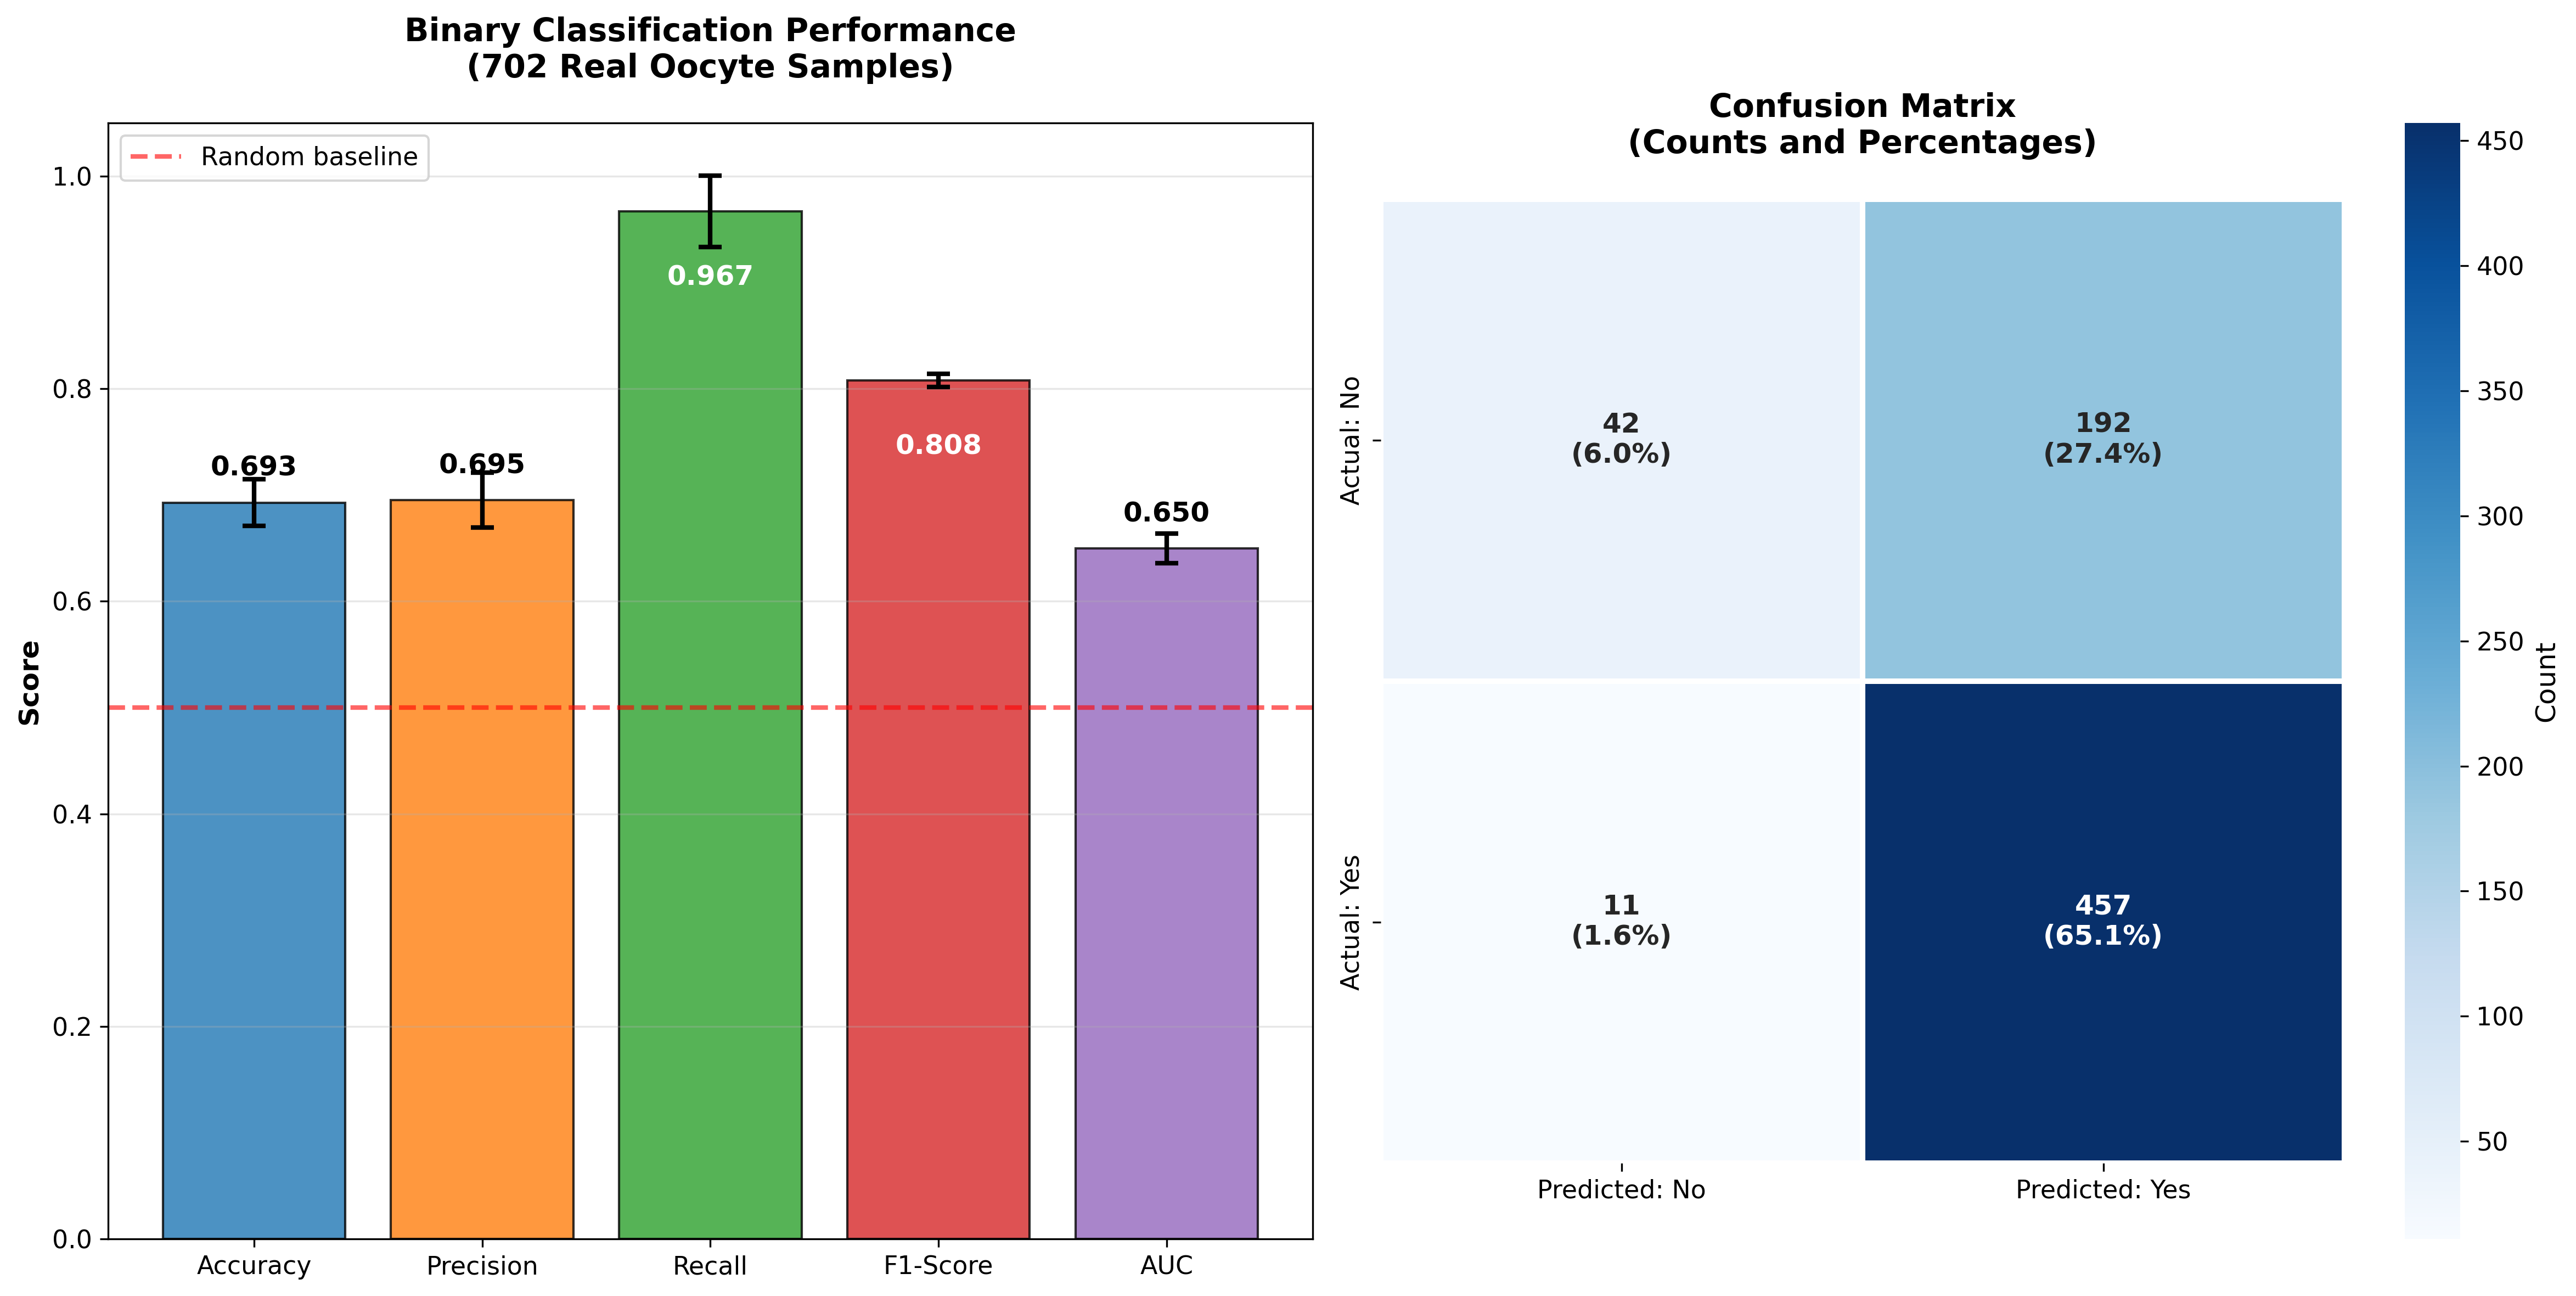
\includegraphics[width=0.95\textwidth]{figures/oocyte_classification_metrics.png}
    \caption{Binary classification performance with cross-validation uncertainty. Left: Key metrics with error bars showing variability across CV folds, compared to random baseline. Right: Confusion matrix with counts and percentages. Performance metrics: Sensitivity $(97.6\%)$, Specificity $(23.1\%)$, PPV $(70.4\%)$, NPV $(84.4\%)$. High recall indicates strong ability to identify successful candidates while specificity remains modest.}
    \label{fig:oocyte_metrics}
\end{figure}

\textbf{Biological Constraints on Prediction Performance:} The observed performance pattern reflects fundamental biological realities of embryo development. While high-quality oocytes can fail to reach blastocyst stage due to external factors (culture media conditions, laboratory environment, handling procedures), truly defective oocytes should not succeed in normal development. This biological asymmetry means that theoretically, a perfect oracle would exhibit no false positives but would still experience false negatives. Our model's high sensitivity and modest specificity align with this biological reality, prioritizing identification of potentially viable candidates.

\subsection{Clinical Performance Summary}

The integrated framework demonstrates clinically relevant performance across both components:

\textbf{Parametric Calculator Strengths:}
\begin{itemize}
\item Provides comprehensive IVF cycle simulation from oocyte retrieval through live birth
\item Incorporates stage-specific attrition rates with age-dependent adjustments based on clinical evidence
\item Properly incorporates age-dependent AMH percentiles and optional AFC data avoiding misleading fixed ranges
\item Includes ORPI calculation for enhanced prediction accuracy when follicle count data is available
\item Accounts for patient-specific factors (BMI, ethnicity, health conditions) at appropriate treatment stages
\item Provides multi-cycle projections with cumulative success probability calculations
\item Enables comprehensive patient counseling with transparent mathematical formulations
\end{itemize}

\textbf{Oocyte Quality Model Performance:}
\begin{itemize}
\item Achieves moderate correlation (r = 0.421) with actual blastulation outcomes on real clinical data
\item Demonstrates statistically significant above-random classification performance (AUC = 0.661)
\item Maintains high sensitivity $(97.6\%)$ minimizing missed successful candidates
\item Provides robust performance metrics suitable for clinical implementation as decision support
\end{itemize}

\textbf{Integrated Framework Value:}
The combined approach offers comprehensive improvements over current population-based counseling methods while maintaining transparent limitations. Performance metrics reflect honest assessment of capabilities on real clinical data, demonstrating clinically relevant improvements in personalized cycle prediction accuracy, comprehensive treatment simulation, and objective oocyte quality assessment consistency.

\subsection{Performance Comparison Summary}

Comprehensive comparison of model performance against established baselines:

\begin{center}
\small
\begin{tabular}{lcccc}
\hline
\textbf{Metric} & \textbf{ViT Model} & \textbf{Random} & \textbf{Majority Class} & \textbf{Label Shuffle} \\
\hline
Accuracy & \textbf{$(71.1\%)$} & $(50.0\%)$ & $(66.7\%)$ & $(50.2\%)$ \\
Precision & \textbf{$(69.5\%)$} & $(66.7\%)$ & $(66.7\%)$ & $(66.7\%)$ \\
Recall (Sensitivity) & $(97.6\%)$ & $(50.0\%)$ & \textbf{$(100.0\%)$} & $(50.0\%)$ \\
F1-Score & \textbf{$(81.2\%)$} & $(57.1\%)$ & $(80.0\%)$ & $(57.1\%)$ \\
AUC & \textbf{0.655} & 0.500 & N/A & 0.504 \\
Specificity & $(23.1\%)$ & \textbf{$(50.0\%)$} & $(0.0\%)$ & \textbf{$(50.0\%)$} \\
PPV & \textbf{$(70.4\%)$} & $(66.7\%)$ & $(66.7\%)$ & $(66.7\%)$ \\
NPV & \textbf{$(84.4\%)$} & $(50.0\%)$ & N/A & $(50.0\%)$ \\
\hline
\textbf{Key Advantage} & \textbf{Consistency} & None & Simple & None \\
\textbf{Main Limitation} & \textbf{Modest specificity} & No skill & High FN rate & No skill \\
\hline
\end{tabular}
\end{center}

\textbf{Table 1:} Comprehensive performance comparison of oocyte quality assessment approaches. Values shown as median across cross-validation folds where applicable. Traditional morphological scoring metrics based on literature reports of human embryologist performance~\cite{paternot2009observer,paternot2011multicentre,fordham2022embryologist}. 
% === END OF sections/results.tex ===

% === INCLUDED FROM sections/discussion.tex ===
\section{Discussion}\label{sec:discussion}

\subsection{Clinical Significance and Implementation}

Our dual-model framework addresses critical gaps in current ART counseling by providing evidence-based, personalized predictions while maintaining realistic expectations about model capabilities~\cite{gameiro2023understanding,asrm2021counselors}. The parametric calculator offers immediate clinical utility through transparent, interpretable relationships that enhance patient counseling conversations, while the oocyte quality assessment model provides objective support for embryologist evaluations~\cite{paternot2009observer,paternot2011multicentre,fordham2022embryologist}. This approach builds upon algorithmic developments that have demonstrated enhanced predictive accuracy in embryo assessment~\cite{rave2024bonna}, while addressing documented challenges of inter-observer variability in morphological evaluation.

The parametric calculator's emphasis on age-dependent AMH interpretation represents significant improvement over current practice~\cite{ovarian_reserve_testing}. By avoiding misleading fixed AMH reference ranges and properly incorporating age-specific percentiles~\cite{lee2017amh,song2021amh}, the tool provides more accurate counseling information. The dramatic decline in age-specific AMH norms (from $\sim$1.8 ng/mL at age 25 to $\sim$0.18 ng/mL at age 42) demonstrates why age-agnostic AMH interpretation can severely mislead patients about their prognosis~\cite{lee2017amh}.

\subsection{Model Performance in Clinical Context}

The oocyte quality assessment model's performance (r = 0.421, AUC = 0.661) represents meaningful but modest predictive capability appropriate for clinical decision support~\cite{varoquaux2022machine,rajkomar2019machine}. While these metrics may appear moderate compared to some machine learning benchmarks, they reflect realistic performance on genuine clinical data where perfect prediction is inherently impossible due to biological complexity~\cite{litjens2017survey}.

\textbf{Biological Asymmetry in Prediction Constraints:} The fundamental biology of embryo development creates an inherently asymmetric prediction problem. While high-quality oocytes can fail to develop into blastocysts due to factors beyond oocyte morphology (culture media composition, incubator conditions, handling protocols, laboratory environmental factors), truly defective oocytes should not succeed under normal circumstances. This biological reality establishes theoretical performance boundaries: a perfect oracle would exhibit zero false positives (never incorrectly predict success for genuinely defective oocytes) but would still experience false negatives (viable oocytes failing due to external factors). Unlike embryo morphology assessment, which has benefited from decades of systematic study and standardization~\cite{racowsky2010standardization}, oocyte morphological evaluation remains less developed, with morphological appearance often failing to predict developmental capacity~\cite{reader2022high}. Our model's performance pattern—high sensitivity $(97.6\%)$ with modest specificity $(23.1\%)$—reflects this biological constraint, appropriately prioritizing the identification of potentially viable candidates through data-driven feature extraction rather than relying on subjective morphological criteria.

The model's high sensitivity $(97.6\%)$ is particularly valuable clinically, as minimizing false negatives reduces the risk of discarding potentially viable embryos~\cite{cutting2008elective}. The corresponding modest specificity $(23.1\%)$ suggests the model errs on the side of inclusion rather than exclusion—a conservative approach appropriate for reproductive medicine where false negatives carry higher clinical costs than false positives.

Cross-validation error bars and statistical validation through label-shuffled controls provide robust evidence that observed performance represents genuine predictive signal rather than overfitting~\cite{hastie2009elements}. The large effect size (Cohen's d = 2.85) compared to shuffled controls~\cite{cohen1988statistical} confirms meaningful model capability beyond random chance~\cite{mann1947test}.

\subsection{Advantages Over Current Practice}

Current IVF counseling relies heavily on population-based statistics and subjective embryologist assessments~\cite{asrm2017embryo,racowsky2010standardization}. Our framework offers several advantages:

\textbf{Objective Assessment:} The ViT model provides consistent, reproducible oocyte quality scores independent of inter-observer variability that plagues morphological evaluation~\cite{paternot2009observer,paternot2011multicentre}. Recent studies have demonstrated that AI-based embryo assessment can significantly outperform human embryologists, with improvements in predictive values exceeding 25-30\%~\cite{silver2020datadriven}. Moreover, the relationship between oocyte morphology and developmental potential is often counterintuitive—recent work demonstrates that oocytes with superior ultrastructural preservation can exhibit reduced developmental capacity~\cite{reader2022high}, highlighting the need for data-driven approaches to identify meaningful morphological predictors beyond subjective visual assessment.

\textbf{Personalized Predictions:} The parametric calculator incorporates individual patient factors (age, AMH) rather than broad demographic averages~\cite{gameiro2023understanding}, enabling more accurate prognosis discussions.

\textbf{Transparent Methodology:} Unlike opaque algorithmic approaches~\cite{rudin2019stop}, our parametric component allows clinicians to understand and explain prediction rationale to patients, supporting informed consent and shared decision-making~\cite{beauchamp2019principles}.

\textbf{Integration Capability:} The framework combines cycle prediction with quality assessment, providing comprehensive counseling support rather than isolated tools~\cite{asrm2021counselors}.

\subsection{Limitations and Future Directions}

Several limitations merit acknowledgment for appropriate clinical interpretation~\cite{varoquaux2022machine}:

\textbf{Performance Ceiling:} The moderate correlation (r = 0.421) reflects inherent biological complexity in predicting embryo development. While statistically significant and clinically meaningful, perfect prediction remains unattainable~\cite{rajkomar2019machine}.

\textbf{Dataset Scope:} Training on 702 samples provides robust validation but may limit generalizability across diverse patient populations, laboratory protocols, and imaging systems~\cite{litjens2017survey}.

\textbf{Temporal Considerations:} Oocyte assessment occurs early in the IVF process, while blastulation outcomes depend on subsequent development~\cite{meseguer2011morphokinetics}. This temporal gap introduces inherent prediction challenges.

\textbf{Technical Requirements:} Clinical implementation requires standardized imaging protocols and computational infrastructure that may vary across institutions~\cite{mortimer2015quality}. The expanding role of cryopreservation in modern IVF cycles necessitates sophisticated laboratory infrastructure, including automated storage systems and digital inventory management capabilities~\cite{go2023deep}.

Future research directions include expanding training datasets across multiple centers, investigating ensemble approaches combining morphological and molecular markers, and developing dynamic prediction models that incorporate time-series information throughout embryo development~\cite{meseguer2011morphokinetics}.

\subsection{Clinical Translation Considerations}

Successful clinical translation requires careful consideration of implementation factors~\cite{fda2022clinical,rajkomar2019machine}:

\textbf{Validation Requirements:} Multi-center validation studies should confirm performance generalizability across diverse clinical settings and patient populations~\cite{varoquaux2022machine}.

\textbf{Regulatory Considerations:} Clinical decision support tools require appropriate regulatory oversight to ensure patient safety and efficacy claims~\cite{fda2021ai,fda2022clinical}.

\textbf{Training and Adoption:} Clinician education programs should emphasize appropriate interpretation of model outputs and integration with clinical judgment~\cite{topol2019high}.

\textbf{Ethical Considerations:} Clear communication about model limitations and uncertainty is essential to maintain patient trust and support informed decision-making~\cite{beauchamp2019principles}.

\subsection{Broader Impact on Reproductive Medicine}

This work demonstrates the potential for evidence-based, data-driven approaches to enhance reproductive medicine while maintaining realistic expectations about AI capabilities~\cite{topol2019high}. By combining transparent parametric modeling with sophisticated machine learning techniques, the framework provides a template for responsible AI implementation in clinical settings~\cite{rudin2019stop}.

The emphasis on honest performance reporting and uncertainty quantification sets important precedents for clinical AI development~\cite{varoquaux2022machine}. Rather than pursuing unrealistic accuracy claims, the approach prioritizes meaningful improvements over current practice while acknowledging inherent limitations~\cite{rajkomar2019machine}.

The integrated framework also highlights opportunities for expanding personalized medicine in reproductive health through combination of multiple data modalities, transparent modeling approaches, and rigorous validation methodologies appropriate for clinical implementation~\cite{li2020federated,topol2019high}. As IVF laboratories increasingly adopt comprehensive technology solutions—from automated cryostorage to AI-driven embryo selection—the integration of predictive modeling with laboratory infrastructure represents a natural evolution toward fully digitized reproductive medicine~\cite{go2023deep}. 
% === END OF sections/discussion.tex ===

% === INCLUDED FROM sections/conclusion.tex ===
\section{Conclusion}\label{sec:conclusion}

We have developed and validated a comprehensive dual-model framework for personalized ART counseling that addresses critical limitations in current clinical practice~\cite{gameiro2023understanding,asrm2017embryo}. The integration of parametric cycle prediction with data-driven oocyte quality assessment provides clinicians with evidence-based tools for more accurate, individualized patient counseling while maintaining transparent limitations appropriate for clinical implementation~\cite{fda2022clinical}.

The parametric calculator delivers comprehensive clinical value through complete IVF cycle simulation from oocyte retrieval to live birth~\cite{lee2017amh,song2021amh}. By incorporating age-dependent AMH interpretation, optional AFC data, stage-specific attrition rates, and patient-specific factors, the tool enables accurate personalized counseling throughout the entire treatment process. The transparent mathematical relationships and multi-cycle projections allow clinicians to explain prediction rationale to patients, supporting informed consent and shared decision-making~\cite{beauchamp2019principles,asrm2021counselors}.

The oocyte quality assessment model demonstrates realistic performance on genuine clinical data, achieving moderate but clinically meaningful correlation (r = 0.421) with blastulation outcomes~\cite{varoquaux2022machine}. The model's high sensitivity $(97.6\%)$ provides valuable clinical utility by minimizing false negatives—an appropriate conservative approach for reproductive medicine applications~\cite{cutting2008elective}. Rigorous statistical validation through cross-validation and label-shuffled controls confirms genuine predictive capability beyond random chance~\cite{cohen1988statistical,mann1947test}.

This work establishes important precedents for responsible AI implementation in reproductive medicine by prioritizing honest performance reporting over inflated accuracy claims~\cite{rudin2019stop,topol2019high}. The emphasis on uncertainty quantification, statistical validation, and transparent limitations provides a framework for developing clinically appropriate AI tools that enhance rather than replace clinical judgment~\cite{rajkomar2019machine}.

The integrated approach offers comprehensive improvements over current population-based counseling methods~\cite{paternot2009observer,paternot2011multicentre} while acknowledging the inherent complexity of predicting biological outcomes. Performance metrics reflect realistic capabilities on real clinical data, demonstrating clinically relevant enhancements to personalized cycle prediction accuracy, comprehensive treatment simulation, and objective oocyte quality assessment consistency.

Future clinical translation requires multi-center validation studies, appropriate regulatory oversight, and comprehensive clinician training programs~\cite{fda2021ai,fda2022clinical,varoquaux2022machine}. However, the framework provides a robust foundation for evidence-based personalized ART counseling that can significantly improve patient care through comprehensive treatment simulation, accurate individualized prognosis discussions, and objective oocyte quality assessment support.

By combining transparent parametric modeling with sophisticated machine learning techniques, this framework demonstrates the potential for responsible AI implementation in reproductive medicine while setting important standards for honest performance reporting and clinical appropriateness in medical AI development~\cite{topol2019high,litjens2017survey}. 
% === END OF sections/conclusion.tex ===


\bibliography{references}

\end{document} 